\documentclass[12pt]{article}
\usepackage[a4paper, margin=1in]{geometry}
\usepackage{graphicx}
\usepackage{lmodern}
\usepackage{setspace}
\usepackage{courier}
\usepackage{xcolor}

\begin{document}
	\title{Clase Práctica 6 - Ordenamiento}
	\author{Juan Ignacio Elosegui}
	\date{Junio 2024}
	\maketitle                   

	\subsection*{Ejercicio 1}
		\begin{itemize}
			\item "Ordenar una secuencia ya ordenada" No es necesario usar ningún algoritmo de ordenamiento previamente visto, ya que la secuencia ya está ordenada. Si quisiéramos ordenarla se podría resolver en O(1).
			\item "Insertar \texttt{k} elementos en su posición en una secuencia \texttt{v} ordenada, con \texttt{k} significativamente mas chico que \texttt{v.size()}" Se puede usar \textbf{Insertion Sort}, porque queremos insertar cada uno de los \texttt{k} elementos en su posición correcta. Vamos a tener una complejidad de O(\texttt{k}$\cdot$\texttt{|v|}), porque en el peor caso, podríamos llegar a recorrer toda la secuencia \texttt{v} hasta encontrar la posición correcta de cada elemento.\\
			También se podría usar una versión de \textbf{Insertion Sort combinado con un ABB} para hacer la tarea que se nos pide. Encontrar la posición para insertar un elemento de \texttt{k} tiene una complejidad de O(\texttt{k}$\cdot \log$\texttt{|v|}), y la inserción en sí tiene una complejidad de O(\texttt{|v|}).
			\item "Encontrar los \texttt{k} elementos más chicos de la secuencia \texttt{v}, con \texttt{k} significativamente más chico que \texttt{|v|}" Primero nos convendría ordenar la secuencia \texttt{v} con \textbf{Selection Sort}, sólo que usando la siguiente modificación: cuando la parte que ya está ordenada tiene el tamaño de \texttt{k}, devolver ese vector, que contendrá los \texttt{k} elementos más chicos de \texttt{v}. Esto tiene una complejidad de O(\texttt{k} $\cdot$ \texttt{|v|}) para el peor caso, ya que va a iterar sólo \texttt{k} veces sobre la secuencia.
				\begin{center}
					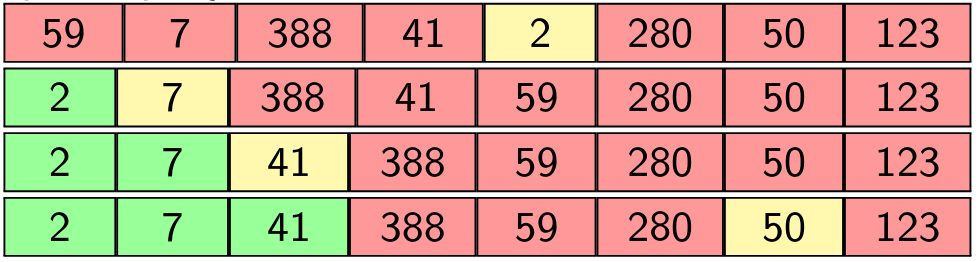
\includegraphics[width=0.6\textwidth]{src/selection_sort.png}\\
					
					Acá sabemos que \texttt{|v|} = 8 y que \texttt{k} = 3 (es decir, queremos los 3 elementos más pequeños de la secuencia). Va a terminar el Selection Sort cuando la subsecuencia verde alcance un tamaño de 3.
				\end{center}
			\item "Dadas dos secuencias ordenadas, devolver una secuencia que
contenga sus elementos ordenados" Acá nos serviría usar sólo la función \textbf{Merge} que se usa comúnmente en el algoritmo de \emph{sorting} de Merge Sort. Si tenemos una secuencia \texttt{m} y otra secuencia \texttt{n}, ambas ordenadas, vamos a tener una complejidad de O(\texttt{|m|+\texttt{|n|}}) en el peor caso.
				\begin{center}
					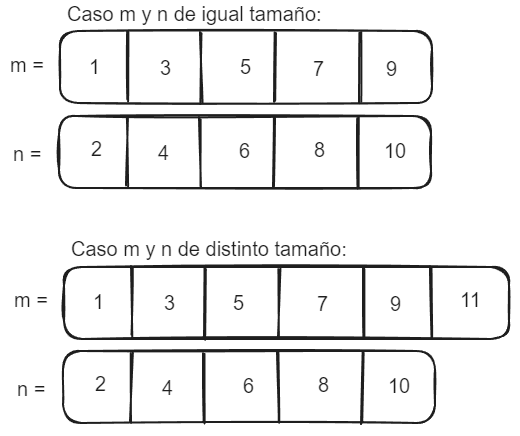
\includegraphics[width=0.4\textwidth]{src/dos_secuencias_ordenadas.png}\\
					
					En ambos casos, se cumple el requerimiento de complejidad en el peor caso.
				\end{center}
			\item "Encontrar los \texttt{k} elementos más grandes de una secuencia \texttt{v}, con \texttt{k} significativamente más chico que \texttt{|v|}" Se puede usar de vuelta el \textbf{Insertion Sort}, que sigue el mismo lineamiento que en el ítem 3, pero queremos devolver la porción de la secuencia que falta. Hay que hacer \texttt{k} iteraciones para encontrar los \texttt{k} elementos más grandes. En cada iteración, encontramos el máximo de la porción de la secuencia que no ha sido ordenada y lo colocamos en su posición correcta.
			\item "Ordenar una secuencia \texttt{v} en el que sus elementos están desordenados en a lo sumo \texttt{k} posiciones, con \texttt{k} significativamente más chico que \texttt{|v|})" Podemos usar de vuelta \textbf{Insertion Sort}, pero sin modificaciones, donde su complejidad es de O(\texttt{k}$\cdot$\texttt{|v|}) en el peor caso.
		\end{itemize}
		
	\subsection*{Ejercicio 2}
			
\end{document}

